\documentclass[10pt,a4paper]{article}

\usepackage[utf8]{inputenc}
\usepackage[T1]{fontenc}
\usepackage[spanish,es-nodecimaldot]{babel}
\usepackage[top=1.5cm,bottom=2cm,left=1.5cm,right=1.5cm]{geometry}
\usepackage{setspace}
\singlespacing
\usepackage{graphicx}
\usepackage{float}
\usepackage{booktabs}
\usepackage{tabularx}
\usepackage{array}
\usepackage{amsmath}
\usepackage{xcolor}
\usepackage{hyperref}
\usepackage{caption}
\usepackage{listings}
\usepackage{parskip}
\usepackage{fancyhdr}

\definecolor{headerdark}{HTML}{2C3E50}
\definecolor{codebackground}{HTML}{F5F5F5}
\definecolor{codecomment}{HTML}{6A9955}
\definecolor{codestring}{HTML}{CE9178}
\definecolor{codekeyword}{HTML}{1F618D}

\hypersetup{
  colorlinks=true,
  linkcolor=headerdark,
  citecolor=headerdark,
  urlcolor=blue!70!black,
  pdftitle={Clasificacion de casos familiares y esporadicos de Neurofibromatosis Tipo 1 mediante Arbol de Decision},
  pdfauthor={Juan Munoz, Vicente Rivera, Fernando Valdes}
}

\captionsetup{font=small,labelfont=bf}
\renewcommand{\figurename}{Fig.}
\renewcommand{\tablename}{Tabla}
\addto\captionsspanish{\renewcommand{\tablename}{Tabla}}
\setlength{\parskip}{3pt}
\setlength{\textfloatsep}{8pt plus 1pt minus 2pt}
\setlength{\floatsep}{6pt plus 1pt minus 2pt}
\renewcommand{\arraystretch}{0.95}

\lstset{
  language=Python,
  backgroundcolor=\color{codebackground},
  basicstyle=\ttfamily\footnotesize,
  breaklines=true,
  frame=single,
  rulecolor=\color{gray!40},
  commentstyle=\color{codecomment},
  stringstyle=\color{codestring},
  keywordstyle=\color{codekeyword}\bfseries,
  numbers=left,
  numberstyle=\tiny\color{gray},
  numbersep=5pt,
  tabsize=2,
  showstringspaces=false,
  captionpos=b,
  literate=
    {á}{{\'a}}1 {é}{{\'e}}1 {í}{{\'i}}1 {ó}{{\'o}}1 {ú}{{\'u}}1
    {Á}{{\'A}}1 {É}{{\'E}}1 {Í}{{\'I}}1 {Ó}{{\'O}}1 {Ú}{{\'U}}1
    {ñ}{{\~n}}1 {Ñ}{{\~N}}1 {ü}{{\"u}}1 {¿}{{?`}}1 {¡}{{!`}}1
}

\begin{document}

\begin{center}
  {\LARGE \textbf{Clasificacion de Casos Familiares y Esporadicos}} \\[3pt]
  {\LARGE \textbf{de Neurofibromatosis Tipo 1 mediante Arbol de Decision}} \\[8pt]
  {\normalsize \textbf{Desarrollado por:} Juan Muñoz, Vicente Rivera, Fernando Valdés} \\[2pt]
  {\small juan.munozveloso2023@alu.uct.cl, vrivera2023@alu.uct.cl, fvaldes2023@alu.uct.cl} \\[2pt]
  {\small \textbf{Ramo:} INFO1184 Inteligencia de Negocios} \\[2pt]
  {\small \textbf{Docente:} Marcos Lévano Humacto} \\[2pt]
  {\small \textbf{Fecha:} 9 de junio de 2026}
\end{center}

\section*{Resumen}

Este informe desarrolla la Tarea 6 de INFO1184 mediante un modelo de arbol de decision aplicado al dataset \textit{Neurofibromatosis Type 1: Clinical Symptoms of Familial and Sporadic Cases}, disponible en el repositorio UCI. El objetivo fue clasificar casos de NF1 como esporadicos o familiares a partir de sintomas clinicos, presencia de tumores y variables de edad, siguiendo CRISP-DM. Se uso el archivo Excel local \texttt{dataset-uci.xlsx}, con 296 registros y 20 columnas; el conjunto presenta 161 casos esporadicos, 135 familiares, 82 pacientes con tumores y valores faltantes solo en edades parentales o edad al primer diagnostico. La preparacion incluyo imputacion por mediana y particion estratificada 75/25. El arbol final se entreno con indice Gini, profundidad maxima 3, minimo de 15 muestras por hoja y ponderacion balanceada. En prueba obtuvo accuracy 0,473, precision 0,447, recall 0,618, F1 0,519 y AUC-ROC 0,521; la validacion cruzada mostro F1 promedio 0,549. Las variables mas influyentes fueron edad al primer diagnostico, nodulos de Lisch, glioma optico y edad de la madre. Los resultados son exploratorios y no constituyen diagnostico medico.

\textbf{Palabras clave:} NF1, arbol de decision, clasificacion, CRISP-DM, Python, UCI.

\tableofcontents

\section{Introduccion}

La neurofibromatosis tipo 1 (NF1) es una condicion genetica asociada a manifestaciones cutaneas, neurologicas, oseas y tumorales. En contextos clinicos y academicos, los registros de sintomas permiten estudiar patrones de presentacion y construir modelos predictivos exploratorios. En este trabajo se analiza el dataset \textit{Neurofibromatosis Type 1: Clinical Symptoms of Familial and Sporadic Cases}, incorporado al repositorio UCI en 2025 y vinculado al estudio de Sharafi et al. sobre prediccion de casos familiares y esporadicos mediante aprendizaje automatico \cite{uci2025nf1,sharafi2025nf1}.

El objetivo general es aplicar el metodo arbol de decision a un problema de clasificacion binaria. La variable objetivo corresponde a \texttt{Case Type}: 0 para caso esporadico y 1 para caso familiar. La variable \texttt{Tumour Case} se mantiene como predictor y tambien se interpreta descriptivamente para discutir diferencias de prevalencia tumoral. La pregunta central es: ¿que sintomas y variables clinicas ayudan a clasificar casos familiares y esporadicos de NF1?

El trabajo se implemento en Python mediante \texttt{pandas}, \texttt{numpy}, \texttt{scikit-learn}, \texttt{matplotlib} y \texttt{seaborn} \cite{pandas2020,sklearn2011,hunter2007,waskom2021}. El proceso completo quedo automatizado en \texttt{nf1\_analisis.py}, que carga datos, prepara variables, entrena el modelo, evalua metricas y genera figuras reproducibles.

\section{Comprension del Negocio}

Desde la perspectiva de inteligencia de negocios aplicada a salud, el problema consiste en transformar registros clinicos de pacientes con NF1 en evidencia interpretable sobre patrones de tipo de caso. La clasificacion familiar/esporadica puede apoyar analisis epidemiologicos, priorizacion de revision genetica y comprension de perfiles clinicos. Sin embargo, el alcance de esta tarea es academico: el modelo no reemplaza evaluacion medica ni asesoramiento genetico.

El criterio de exito no se limita a obtener una metrica alta. Dado que el dataset es pequeno y los sintomas pueden solaparse entre grupos, se busca un flujo metodologico trazable, visualizaciones claras, una evaluacion honesta y una interpretacion prudente. CRISP-DM organiza el trabajo en comprension del negocio, comprension de datos, preparacion, modelado, evaluacion y comunicacion de resultados \cite{chapman2000}.

\begin{table}[H]
\centering
\small
\begin{tabularx}{\textwidth}{p{3.2cm}X}
\toprule
Etapa CRISP-DM & Aplicacion en TA06 \\
\midrule
Comprension del negocio & Clasificar casos de NF1 como familiares o esporadicos usando sintomas clinicos. \\
Comprension de datos & Revisar dimensiones, variables, clases, faltantes, duplicados y prevalencia de sintomas. \\
Preparacion de datos & Separar \texttt{Case Type}, eliminar ID, imputar edades y dividir train/test estratificado. \\
Modelado & Entrenar un arbol de decision interpretable con poda previa y ponderacion balanceada. \\
Evaluacion & Reportar accuracy, precision, recall, F1, AUC-ROC, matriz de confusion y validacion cruzada. \\
Comunicacion & Documentar hallazgos, limitaciones y reproducibilidad en informe, figuras y README. \\
\bottomrule
\end{tabularx}
\caption{Aplicacion de CRISP-DM en el analisis NF1.}
\label{tab:crispdm}
\end{table}

\section{Comprension de los Datos}

El archivo usado fue \texttt{dataset-uci.xlsx}, ubicado en \texttt{TA06/}. La hoja \texttt{Dataset} contiene 296 registros y 20 columnas. La descripcion UCI menciona 331 probandos, pero el Excel local disponible para la tarea contiene 296 filas efectivas; esta diferencia se mantiene documentada para reproducibilidad. La Tabla~\ref{tab:estructura_datos} resume la estructura principal.

\begin{table}[H]
\centering
\begin{tabular}{lr}
\toprule
Indicador & Valor \\
\midrule
Registros en Excel local & 296 \\
Columnas totales & 20 \\
Variable objetivo & \texttt{Case Type} \\
Casos esporadicos & 161 \\
Casos familiares & 135 \\
Pacientes sin tumores & 214 \\
Pacientes con tumores & 82 \\
Duplicados exactos & 0 \\
\bottomrule
\end{tabular}
\caption{Resumen estructural del dataset NF1 usado.}
\label{tab:estructura_datos}
\end{table}

La Fig.~\ref{fig:distribucion_clases} muestra que la variable objetivo esta moderadamente balanceada: 54,4\% de casos esporadicos y 45,6\% familiares. Esto permite usar una particion estratificada y metricas por clase, aunque sigue siendo necesario revisar precision, recall y F1 porque el objetivo positivo corresponde a la clase familiar.

\begin{figure}[H]
\centering
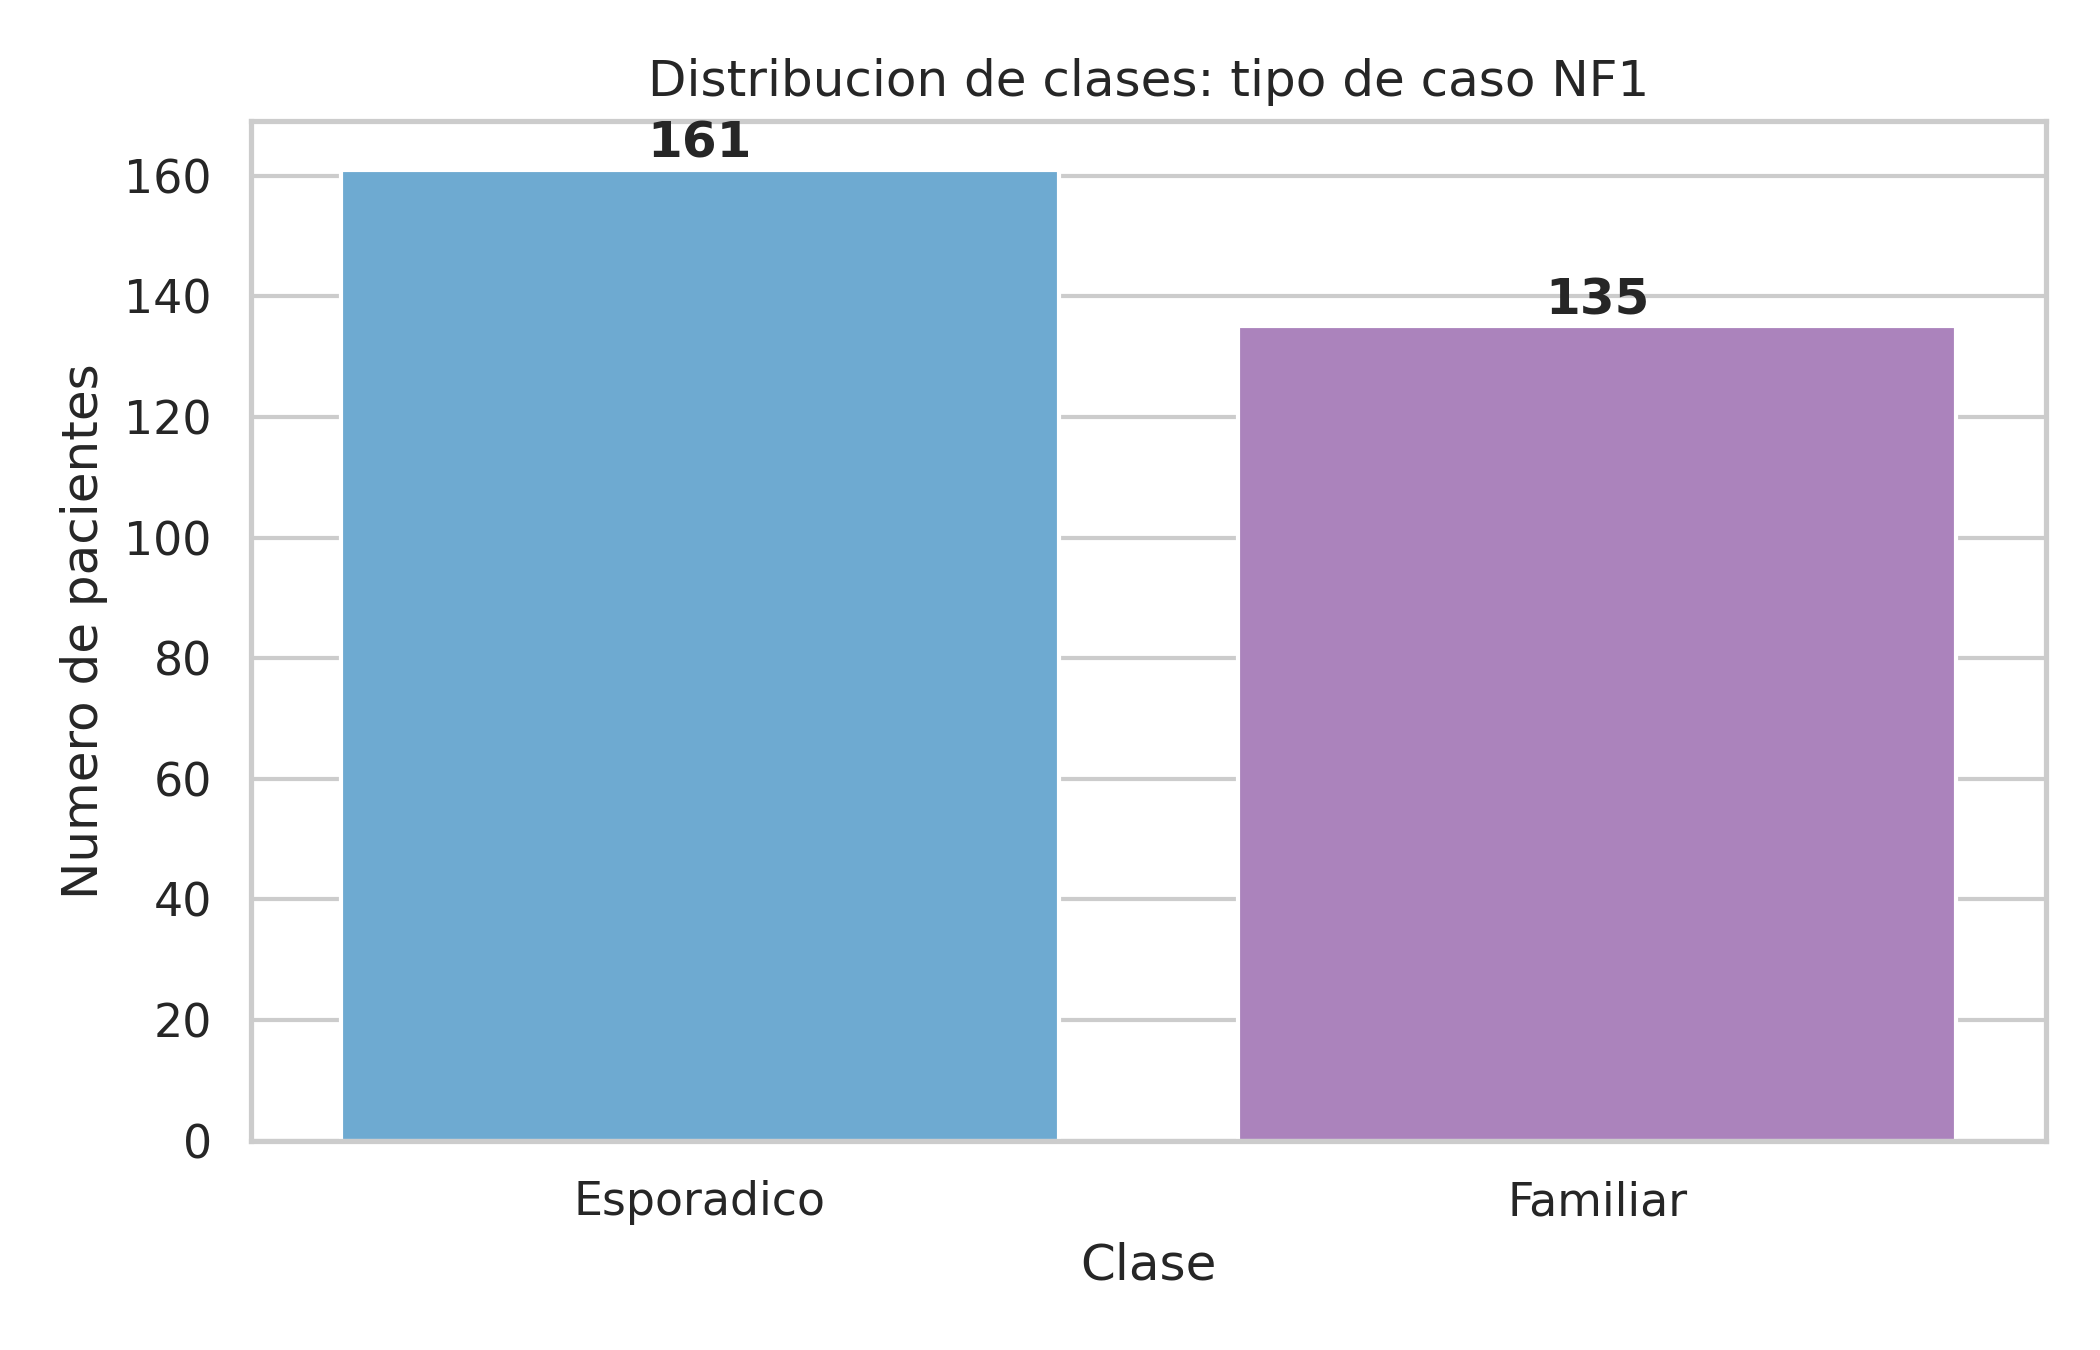
\includegraphics[width=0.58\textwidth]{figuras/distribucion_clases.png}
\caption{Distribucion de clases de la variable objetivo \texttt{Case Type}.}
\label{fig:distribucion_clases}
\end{figure}

Las variables predictoras incluyen presencia de tumores, edad de la madre, edad del padre, edad al primer diagnostico y sintomas binarios como manchas cafe con leche, pecas axilares, pecas inguinales, nodulos de Lisch, neurofibromas, glioma optico, displasia esqueletica, discapacidad de aprendizaje, hipertension, astrocitoma, hamartoma, escoliosis y otros sintomas. Las tres variables de edad presentan valores faltantes: 35 en edad de la madre, 34 en edad del padre y 4 en edad al primer diagnostico.

\begin{table}[H]
\centering
\small
\begin{tabular}{lrrrrr}
\toprule
Variable & n valido & Media & Mediana & Min. & Max. \\
\midrule
Edad de la madre & 261 & 27,18 & 27,00 & 16,00 & 45,00 \\
Edad del padre & 262 & 31,88 & 31,00 & 19,00 & 62,00 \\
Edad al primer diagnostico & 292 & 11,88 & 9,00 & 0,50 & 61,00 \\
\bottomrule
\end{tabular}
\caption{Estadisticas descriptivas de variables de edad.}
\label{tab:edades}
\end{table}

En prevalencia general, las manifestaciones mas frecuentes fueron \texttt{Cafe au lait (CLS)} con 93,2\%, pecas axilares con 53,4\%, otros sintomas con 34,1\%, nodulos de Lisch con 28,0\%, presencia de tumores con 27,7\% y neurofibromas dermales con 27,7\%. La Fig.~\ref{fig:prevalencia_sintomas} compara prevalencias por tipo de caso.

\begin{figure}[H]
\centering
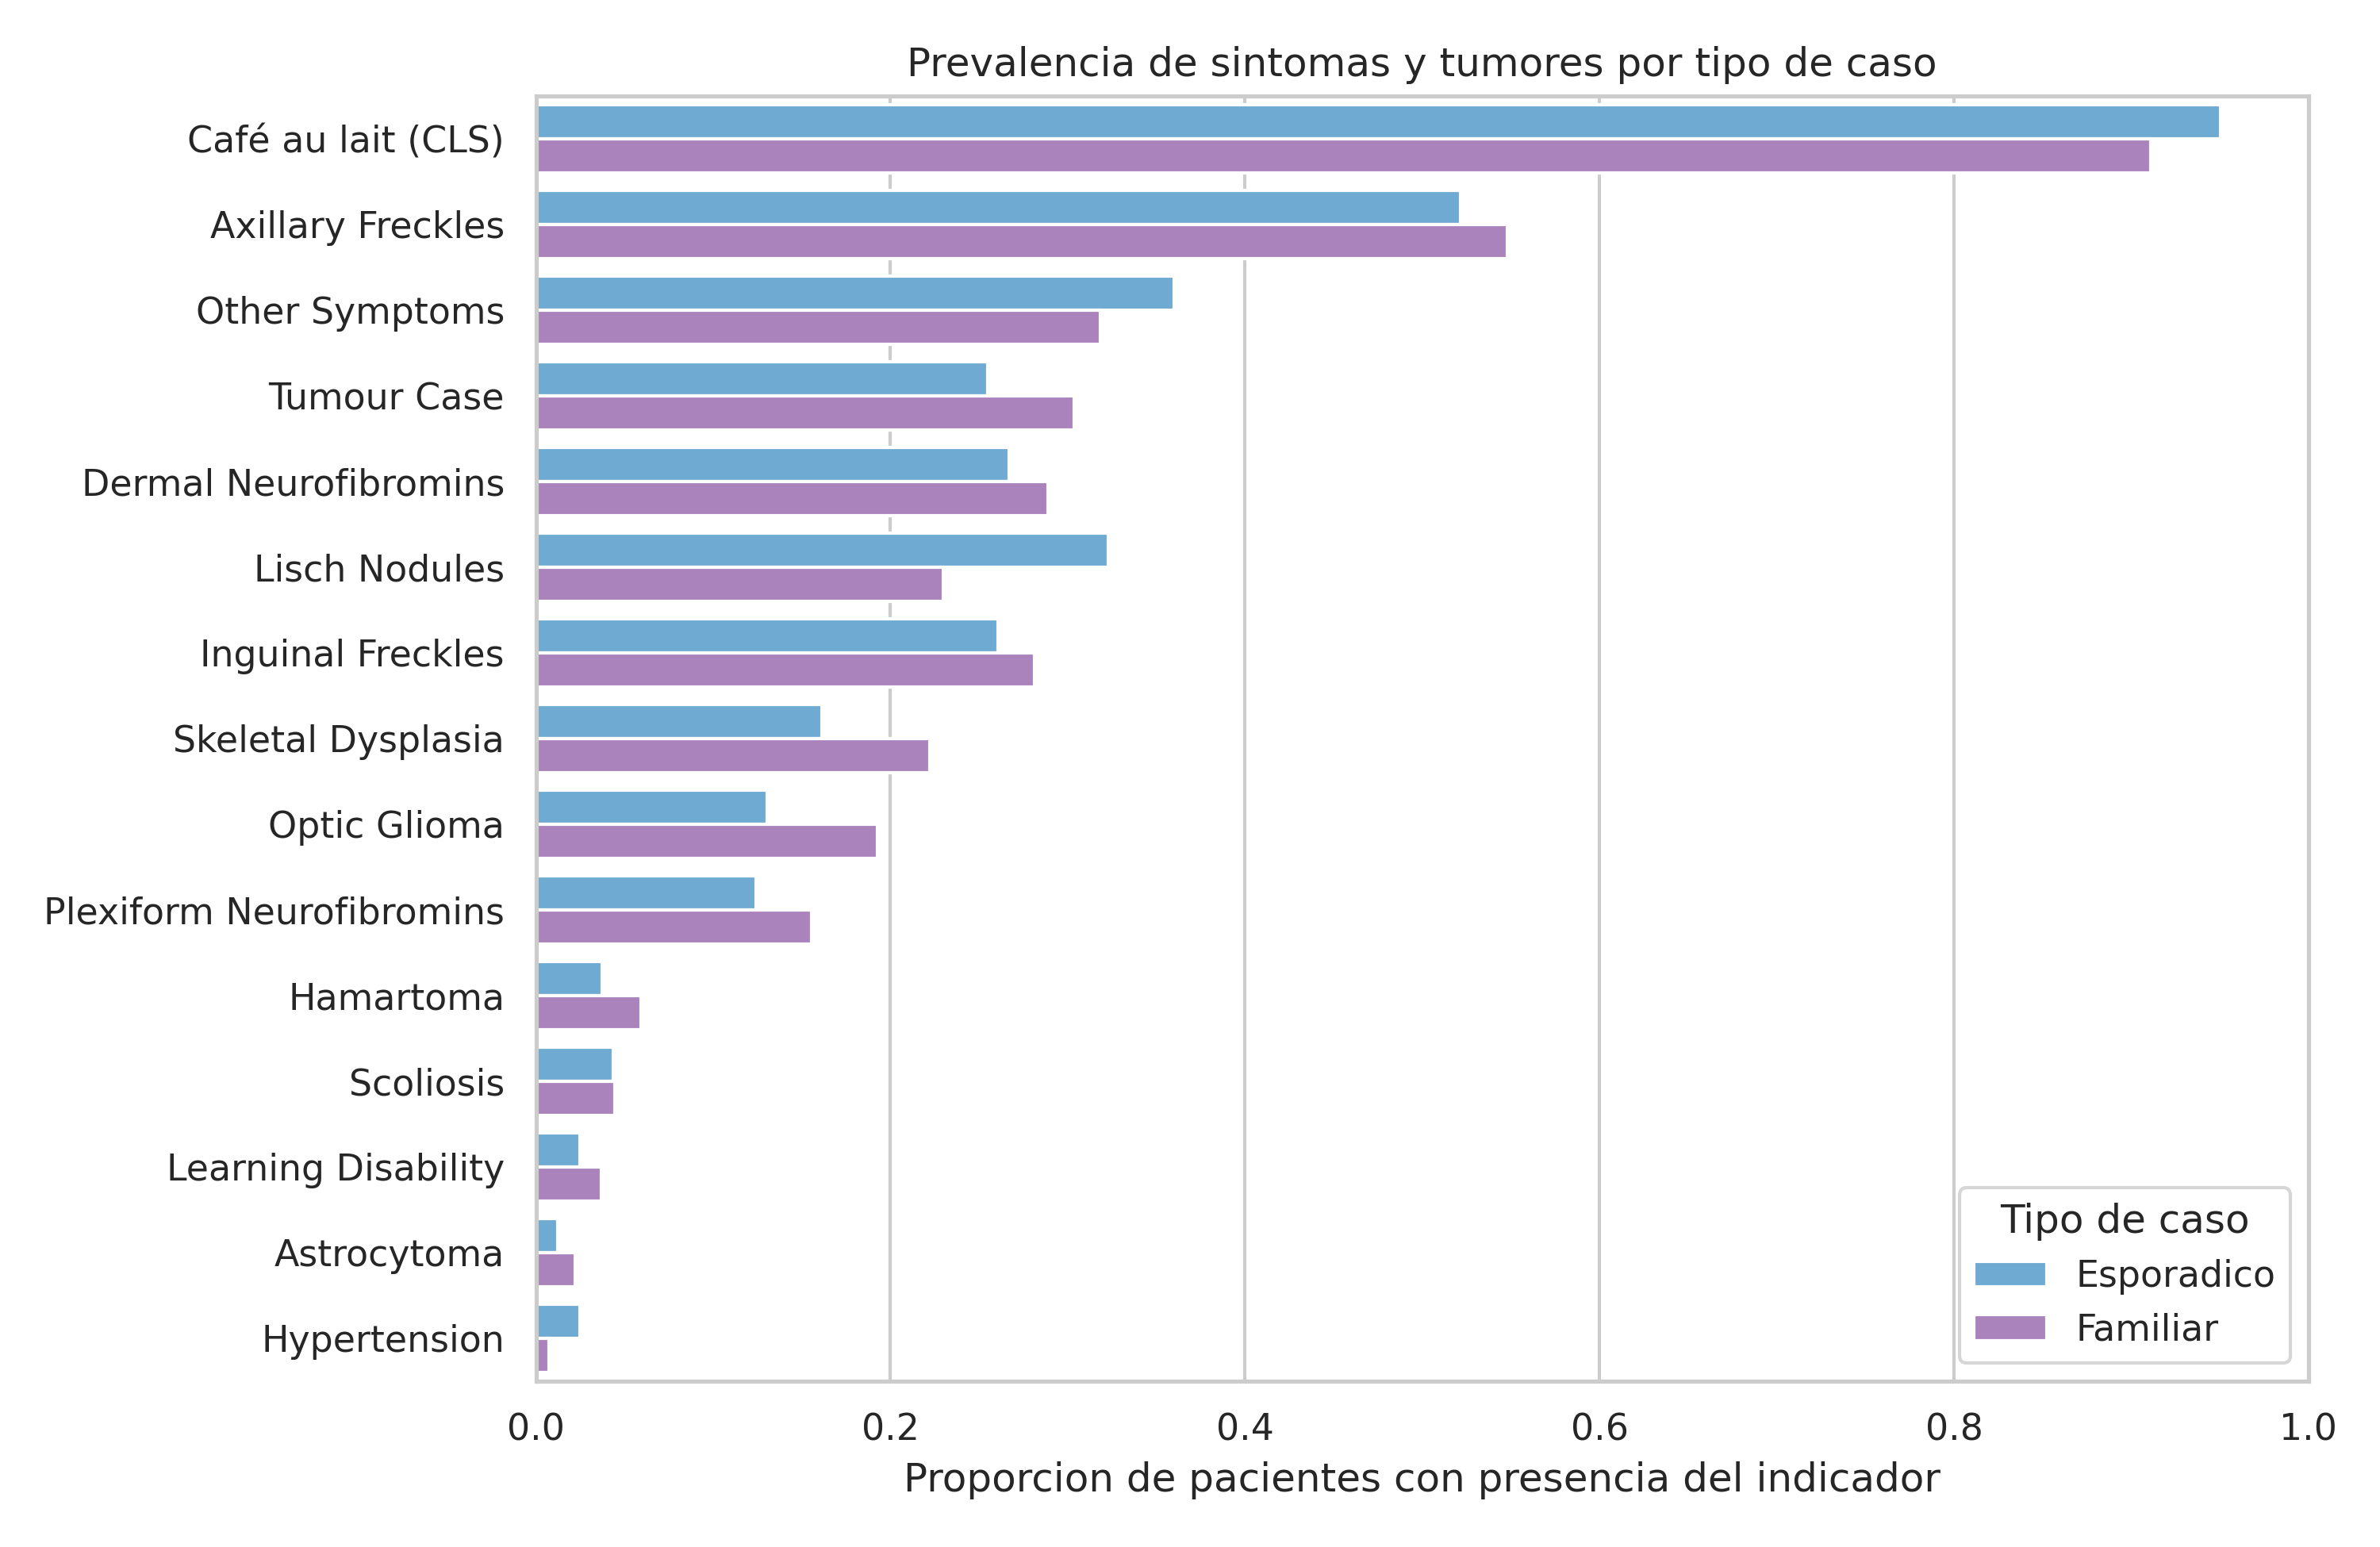
\includegraphics[width=0.86\textwidth]{figuras/prevalencia_sintomas.png}
\caption{Prevalencia de sintomas y tumores por tipo de caso NF1.}
\label{fig:prevalencia_sintomas}
\end{figure}

La diferencia descriptiva mas visible fue que nodulos de Lisch aparecieron mas en casos esporadicos (32,3\%) que familiares (23,0\%). En cambio, glioma optico fue mas frecuente en familiares (19,3\%) que esporadicos (13,0\%), displasia esqueletica tambien fue mayor en familiares (22,2\% frente a 16,1\%) y la presencia de tumores subio de 25,5\% en esporadicos a 30,4\% en familiares. Estas diferencias son utiles para exploracion, pero no implican causalidad clinica.

\section{Preparacion de los Datos}

La preparacion mantuvo el archivo original sin modificar. En el script se elimino la columna identificadora \texttt{ID}, se separo \texttt{Case Type} como variable objetivo y se convirtieron las variables predictoras a formato numerico. Las variables binarias ya estaban codificadas como 0 para ausencia y 1 para presencia. Las edades se imputaron con la mediana, estrategia simple y robusta frente a asimetria moderada.

\begin{lstlisting}[caption={Preparacion principal de variables en Python.}]
target = "Case Type"
df_modelo = df.drop(columns=["ID"])
y = df_modelo[target].astype(int)
X = df_modelo.drop(columns=[target])

variables_edad = [
    "Age of Mother",
    "Age of Father",
    "Age at First Diagnosis",
]
\end{lstlisting}

La division de datos uso 75\% para entrenamiento y 25\% para prueba, con estratificacion por clase y semilla 1184. Ademas, se aplico validacion cruzada estratificada de cinco pliegues para estimar estabilidad y evitar depender solo de una particion.

\section{Modelado}

El arbol de decision es un modelo supervisado que divide recursivamente los datos mediante reglas del tipo ``si una variable cumple una condicion, avanzar por una rama''. Cada nodo busca separar las clases de forma mas pura que el nodo anterior. En CART, el criterio clasico es el indice de Gini \cite{breiman1984}:

\begin{equation}
Gini = 1 - \sum_{i=1}^{k} p_i^2,
\end{equation}

donde $p_i$ es la proporcion de la clase $i$ en el nodo. Un valor 0 indica pureza completa. Otra alternativa es la entropia, asociada a ganancia de informacion:

\begin{equation}
H = -\sum_{i=1}^{k} p_i \log_2(p_i).
\end{equation}

En este trabajo se uso \texttt{DecisionTreeClassifier} de \texttt{scikit-learn}. Para controlar sobreajuste se limito la profundidad maxima a 3, se exigieron al menos 15 observaciones por hoja y se uso \texttt{class\_weight="balanced"}, porque interesa que el modelo no ignore la clase familiar. El preprocesamiento y el modelo se integraron en un \texttt{Pipeline}.

\begin{lstlisting}[caption={Pipeline de modelado usado en el script.}]
preprocesador = ColumnTransformer(
    transformers=[("edad", SimpleImputer(strategy="median"), variables_edad)],
    remainder="passthrough",
    verbose_feature_names_out=False,
)

modelo = DecisionTreeClassifier(
    criterion="gini",
    max_depth=3,
    min_samples_leaf=15,
    class_weight="balanced",
    random_state=1184,
)
\end{lstlisting}

La Fig.~\ref{fig:arbol_decision} presenta el arbol final. Sus reglas principales se concentran en edad al primer diagnostico, nodulos de Lisch, glioma optico y edad de la madre, lo que coincide con el ranking de importancia.

\begin{figure}[H]
\centering
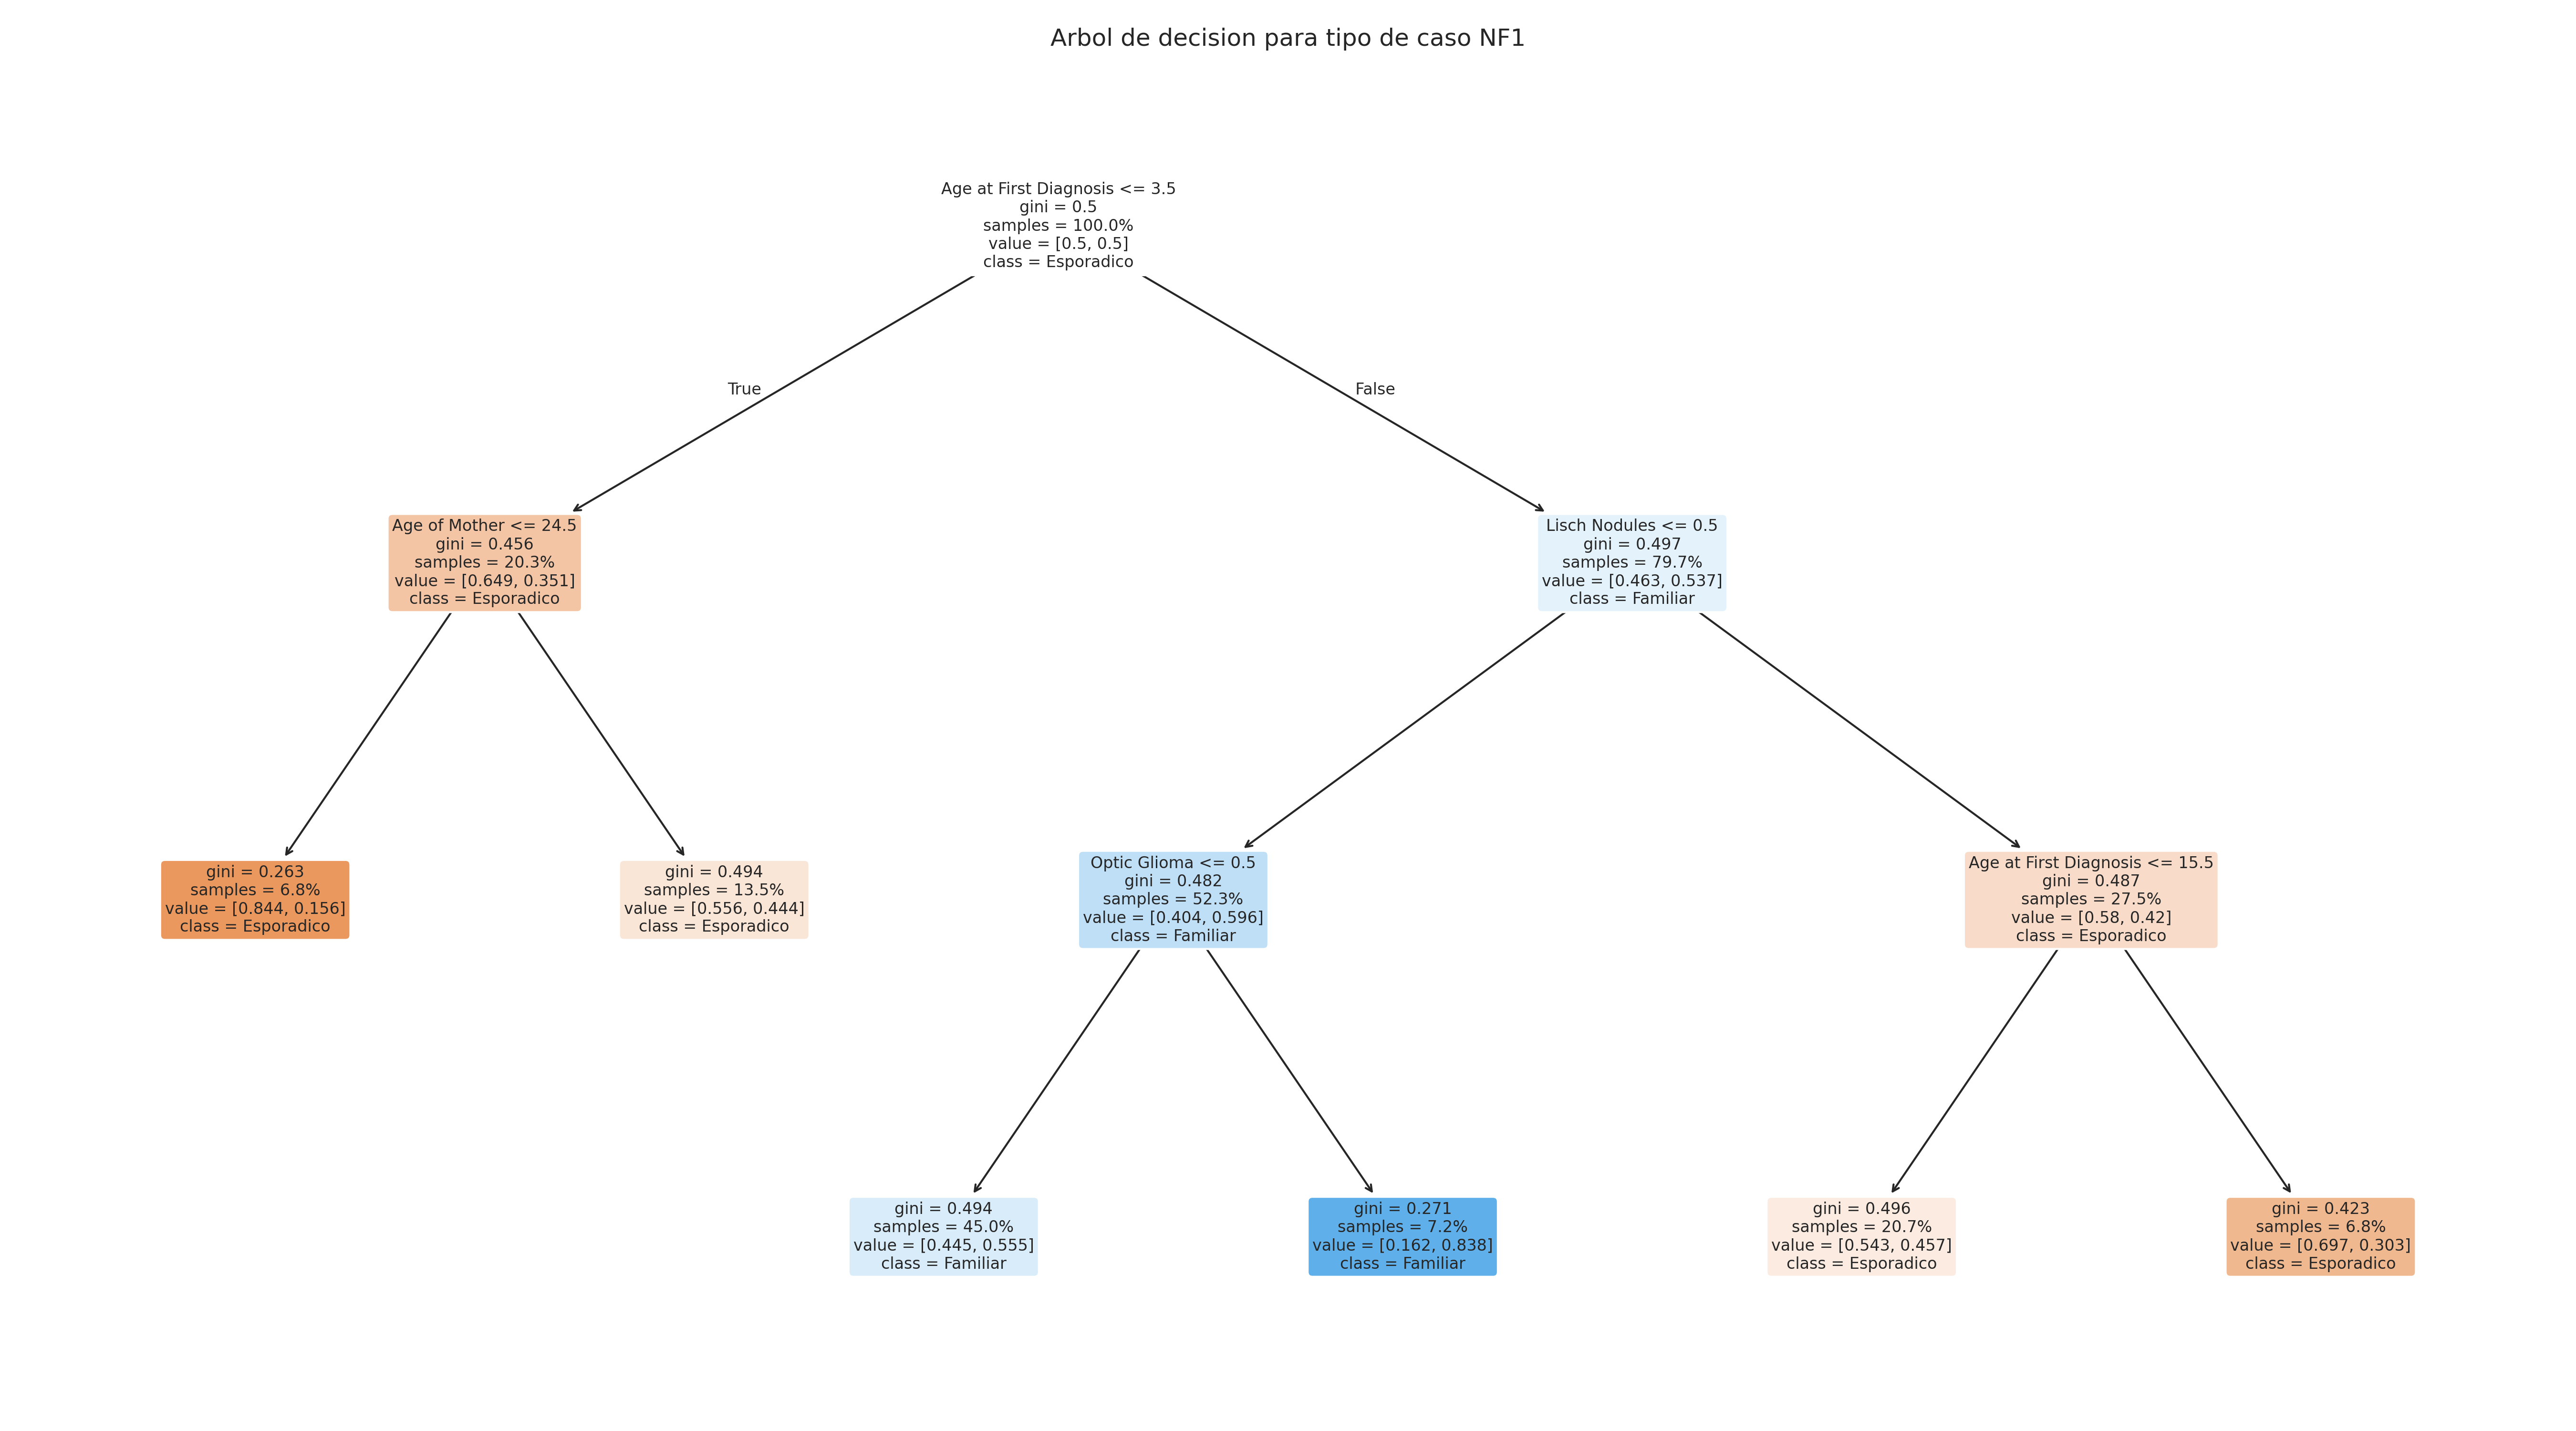
\includegraphics[width=\textwidth]{figuras/arbol_decision.png}
\caption{Arbol de decision entrenado para clasificar casos familiares y esporadicos.}
\label{fig:arbol_decision}
\end{figure}

La Fig.~\ref{fig:importancia_features} resume la importancia relativa de variables. Las cinco primeras fueron edad al primer diagnostico (0,315), nodulos de Lisch (0,263), glioma optico (0,251), edad de la madre (0,171) y edad del padre (0,000). Que varias variables queden en cero no significa irrelevancia clinica absoluta; significa que el arbol final podado no las uso para sus divisiones.

\begin{figure}[H]
\centering
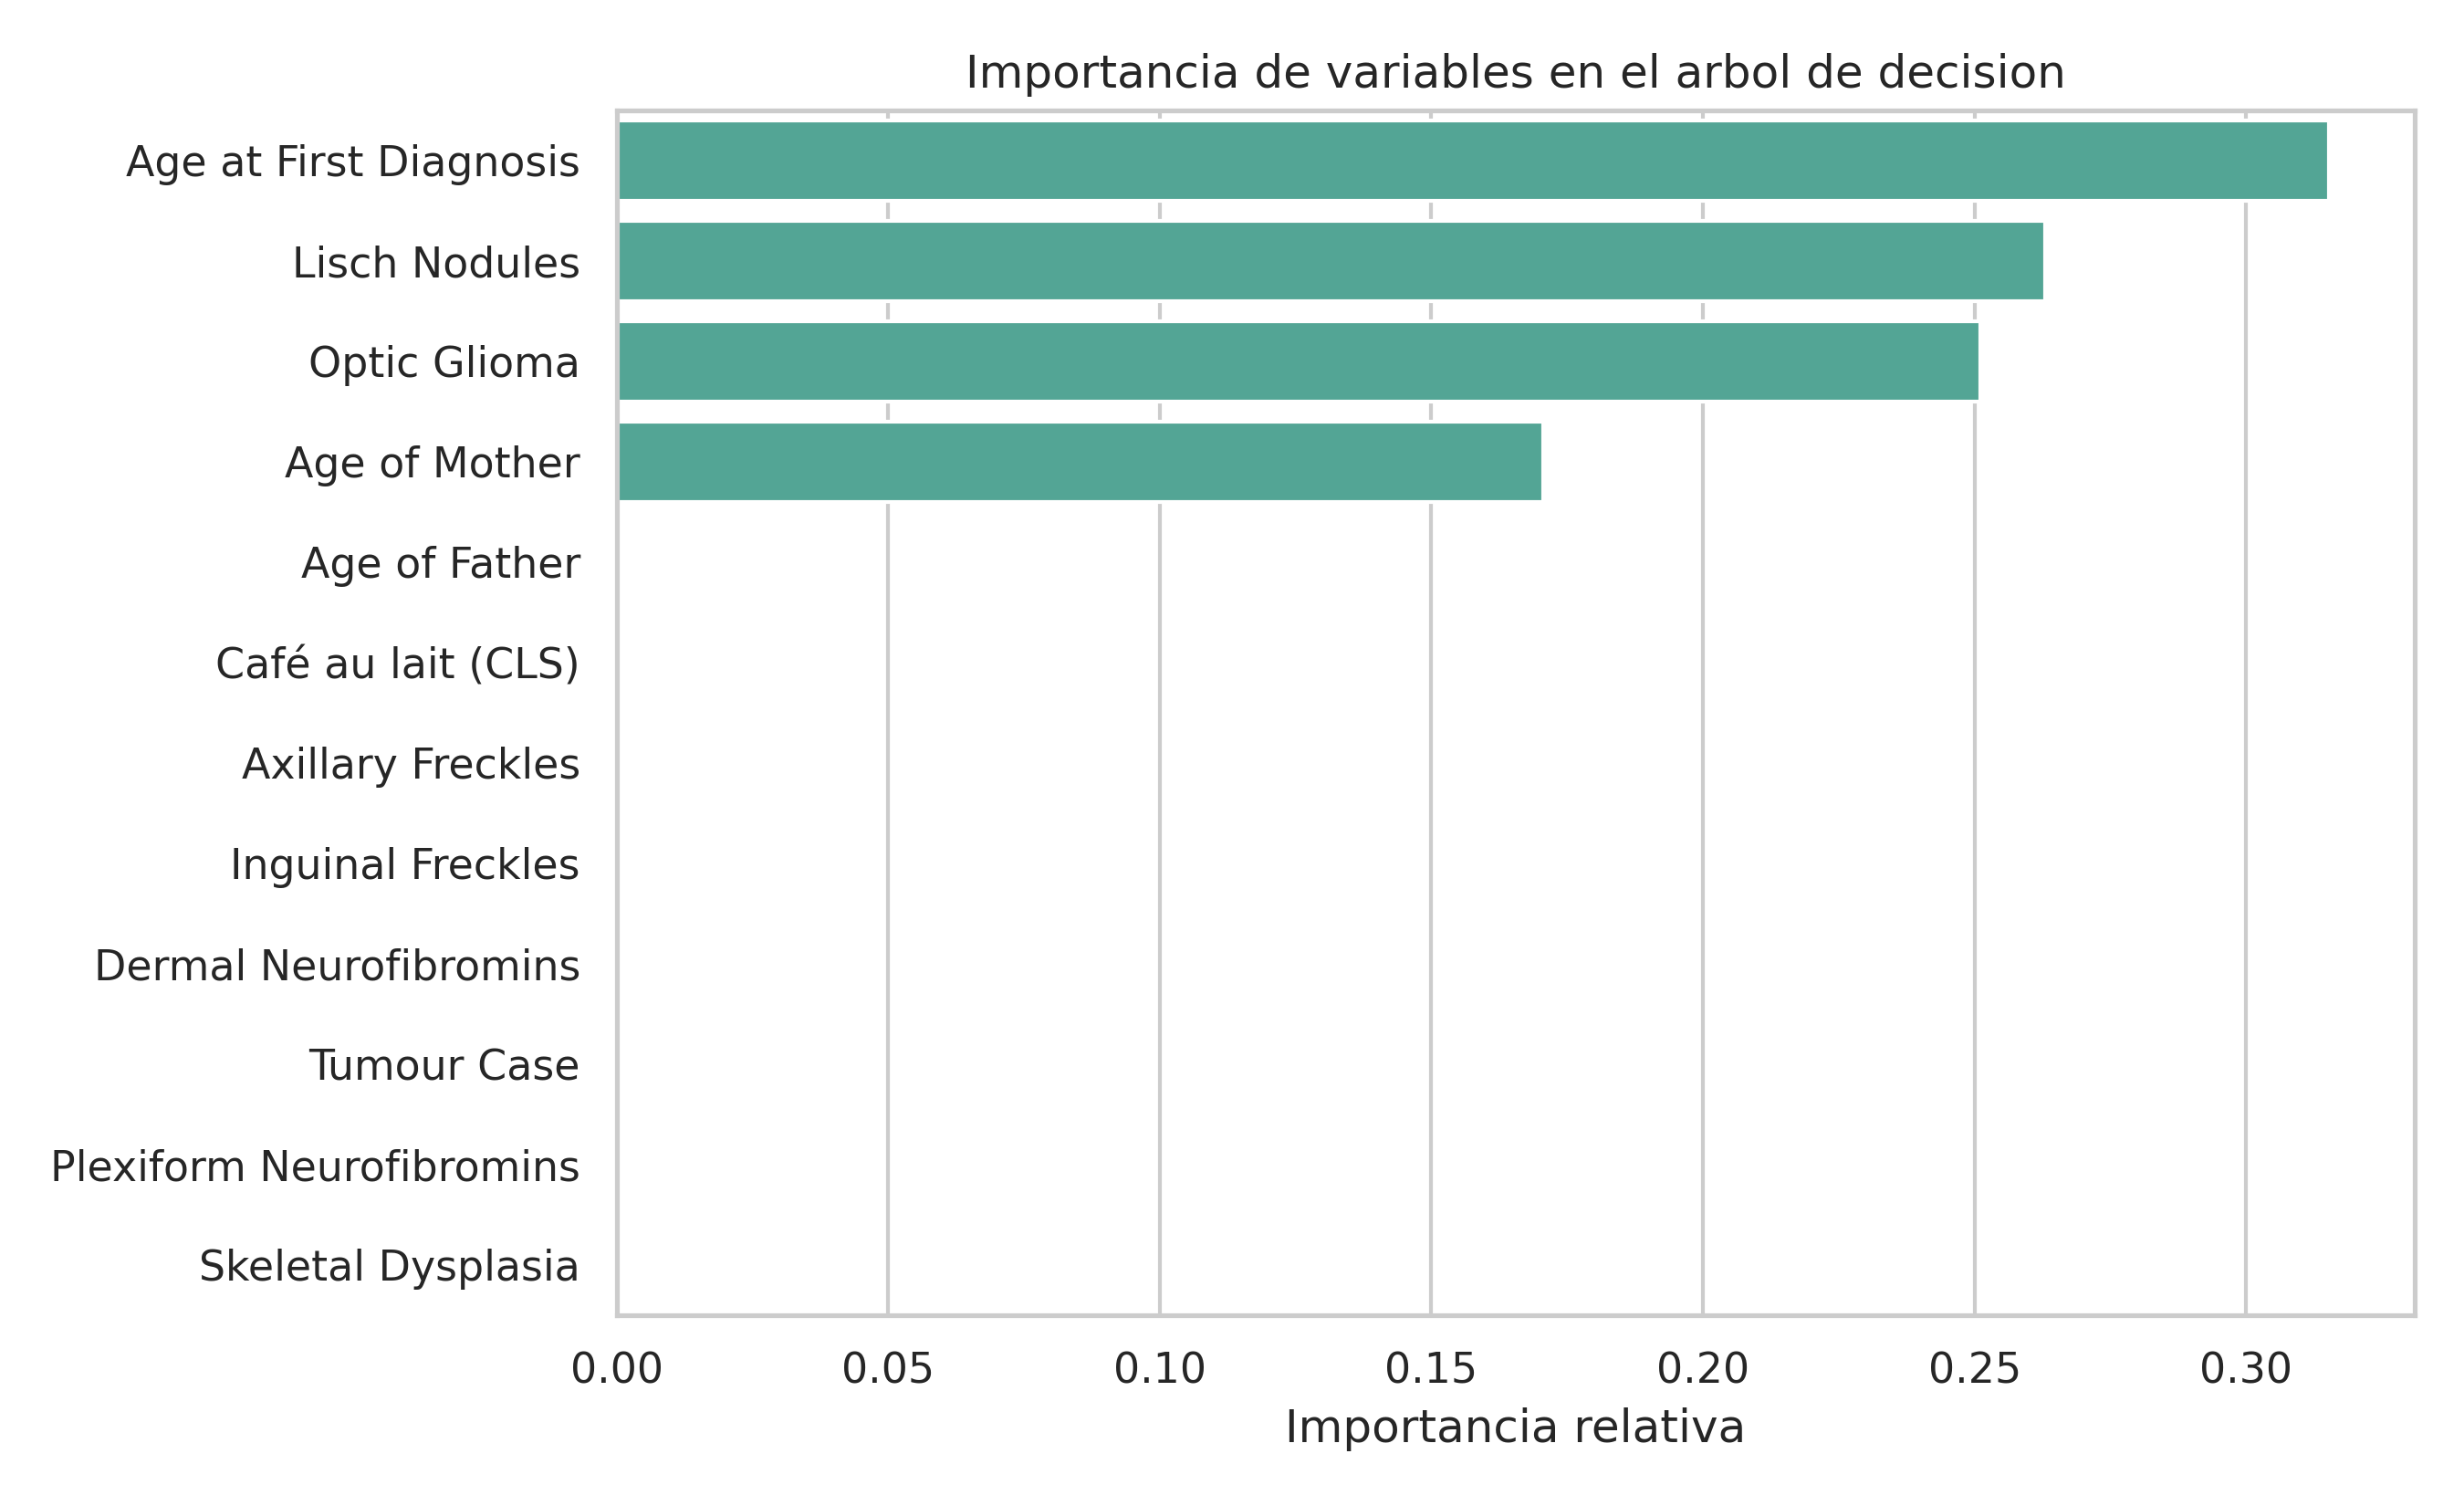
\includegraphics[width=0.76\textwidth]{figuras/importancia_features.png}
\caption{Importancia de variables en el arbol de decision.}
\label{fig:importancia_features}
\end{figure}

\section{Evaluacion}

La evaluacion se realizo en el conjunto de prueba y mediante validacion cruzada. Las metricas usadas fueron accuracy, precision, recall, F1 y AUC-ROC. Para la clase positiva se considero \texttt{Case Type = 1}, es decir, caso familiar.

\begin{table}[H]
\centering
\begin{tabular}{lr}
\toprule
Metrica en test & Valor \\
\midrule
Accuracy & 0,473 \\
Precision clase familiar & 0,447 \\
Recall clase familiar & 0,618 \\
F1-score clase familiar & 0,519 \\
AUC-ROC & 0,521 \\
\bottomrule
\end{tabular}
\caption{Metricas del arbol de decision en conjunto de prueba.}
\label{tab:metricas_test}
\end{table}

La matriz de confusion de la Fig.~\ref{fig:matriz_confusion} muestra 14 esporadicos correctamente identificados, 26 esporadicos clasificados como familiares, 21 familiares correctamente identificados y 13 familiares clasificados como esporadicos. El modelo privilegia recuperar casos familiares, pero al hacerlo aumenta falsos positivos.

\begin{figure}[H]
\centering
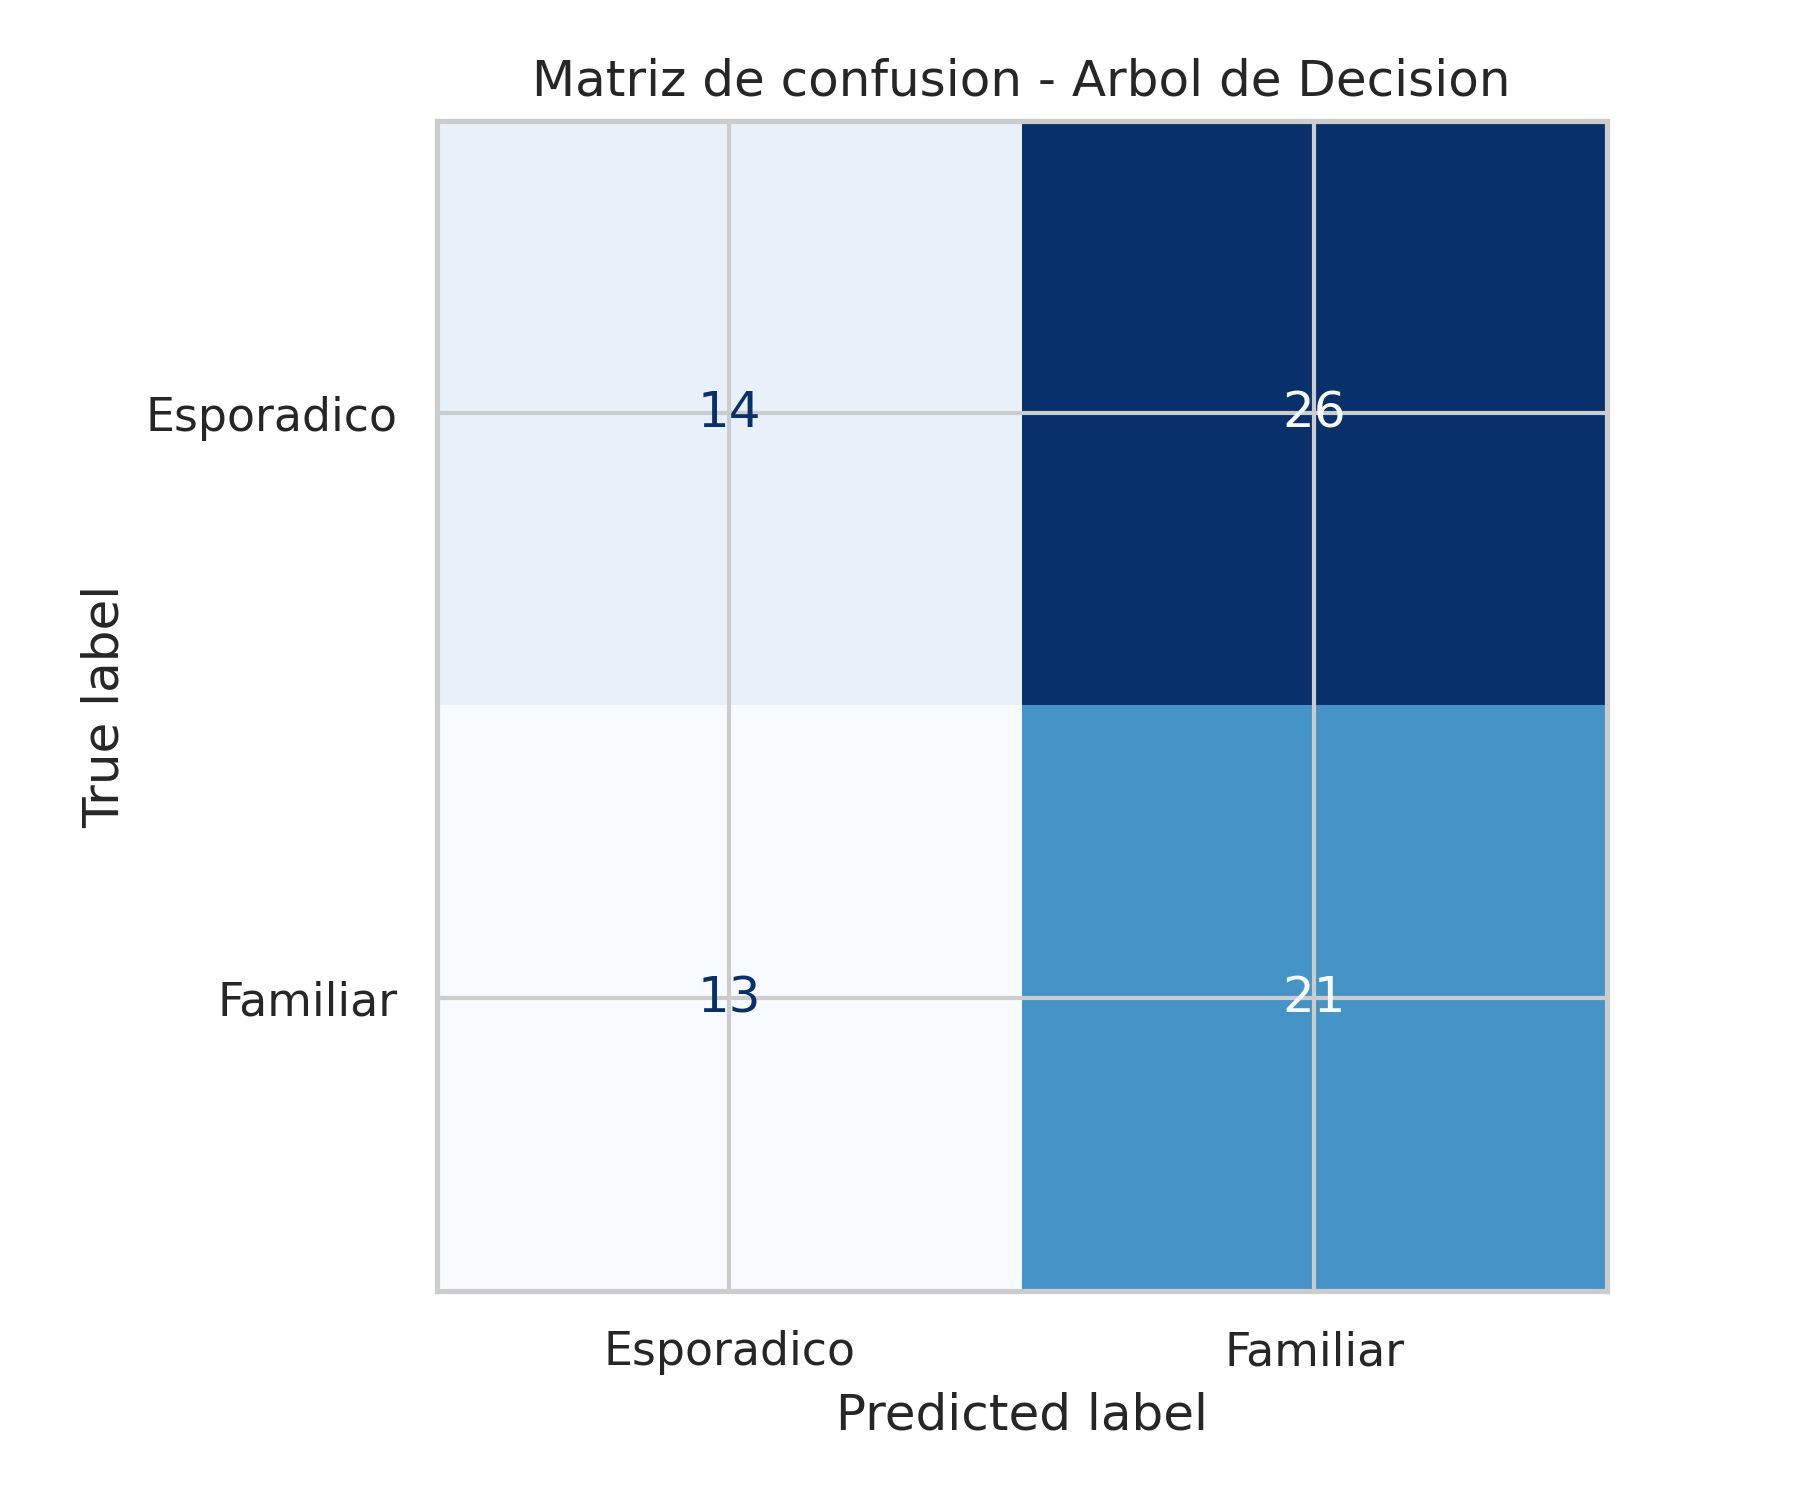
\includegraphics[width=0.56\textwidth]{figuras/matriz_confusion.png}
\caption{Matriz de confusion del arbol de decision en el conjunto de prueba.}
\label{fig:matriz_confusion}
\end{figure}

La curva ROC de la Fig.~\ref{fig:curva_roc} confirma una separacion limitada entre clases. Un AUC de 0,521 esta apenas sobre el azar, por lo que el modelo debe entenderse como ejercicio interpretable y no como clasificador clinico robusto.

\begin{figure}[H]
\centering
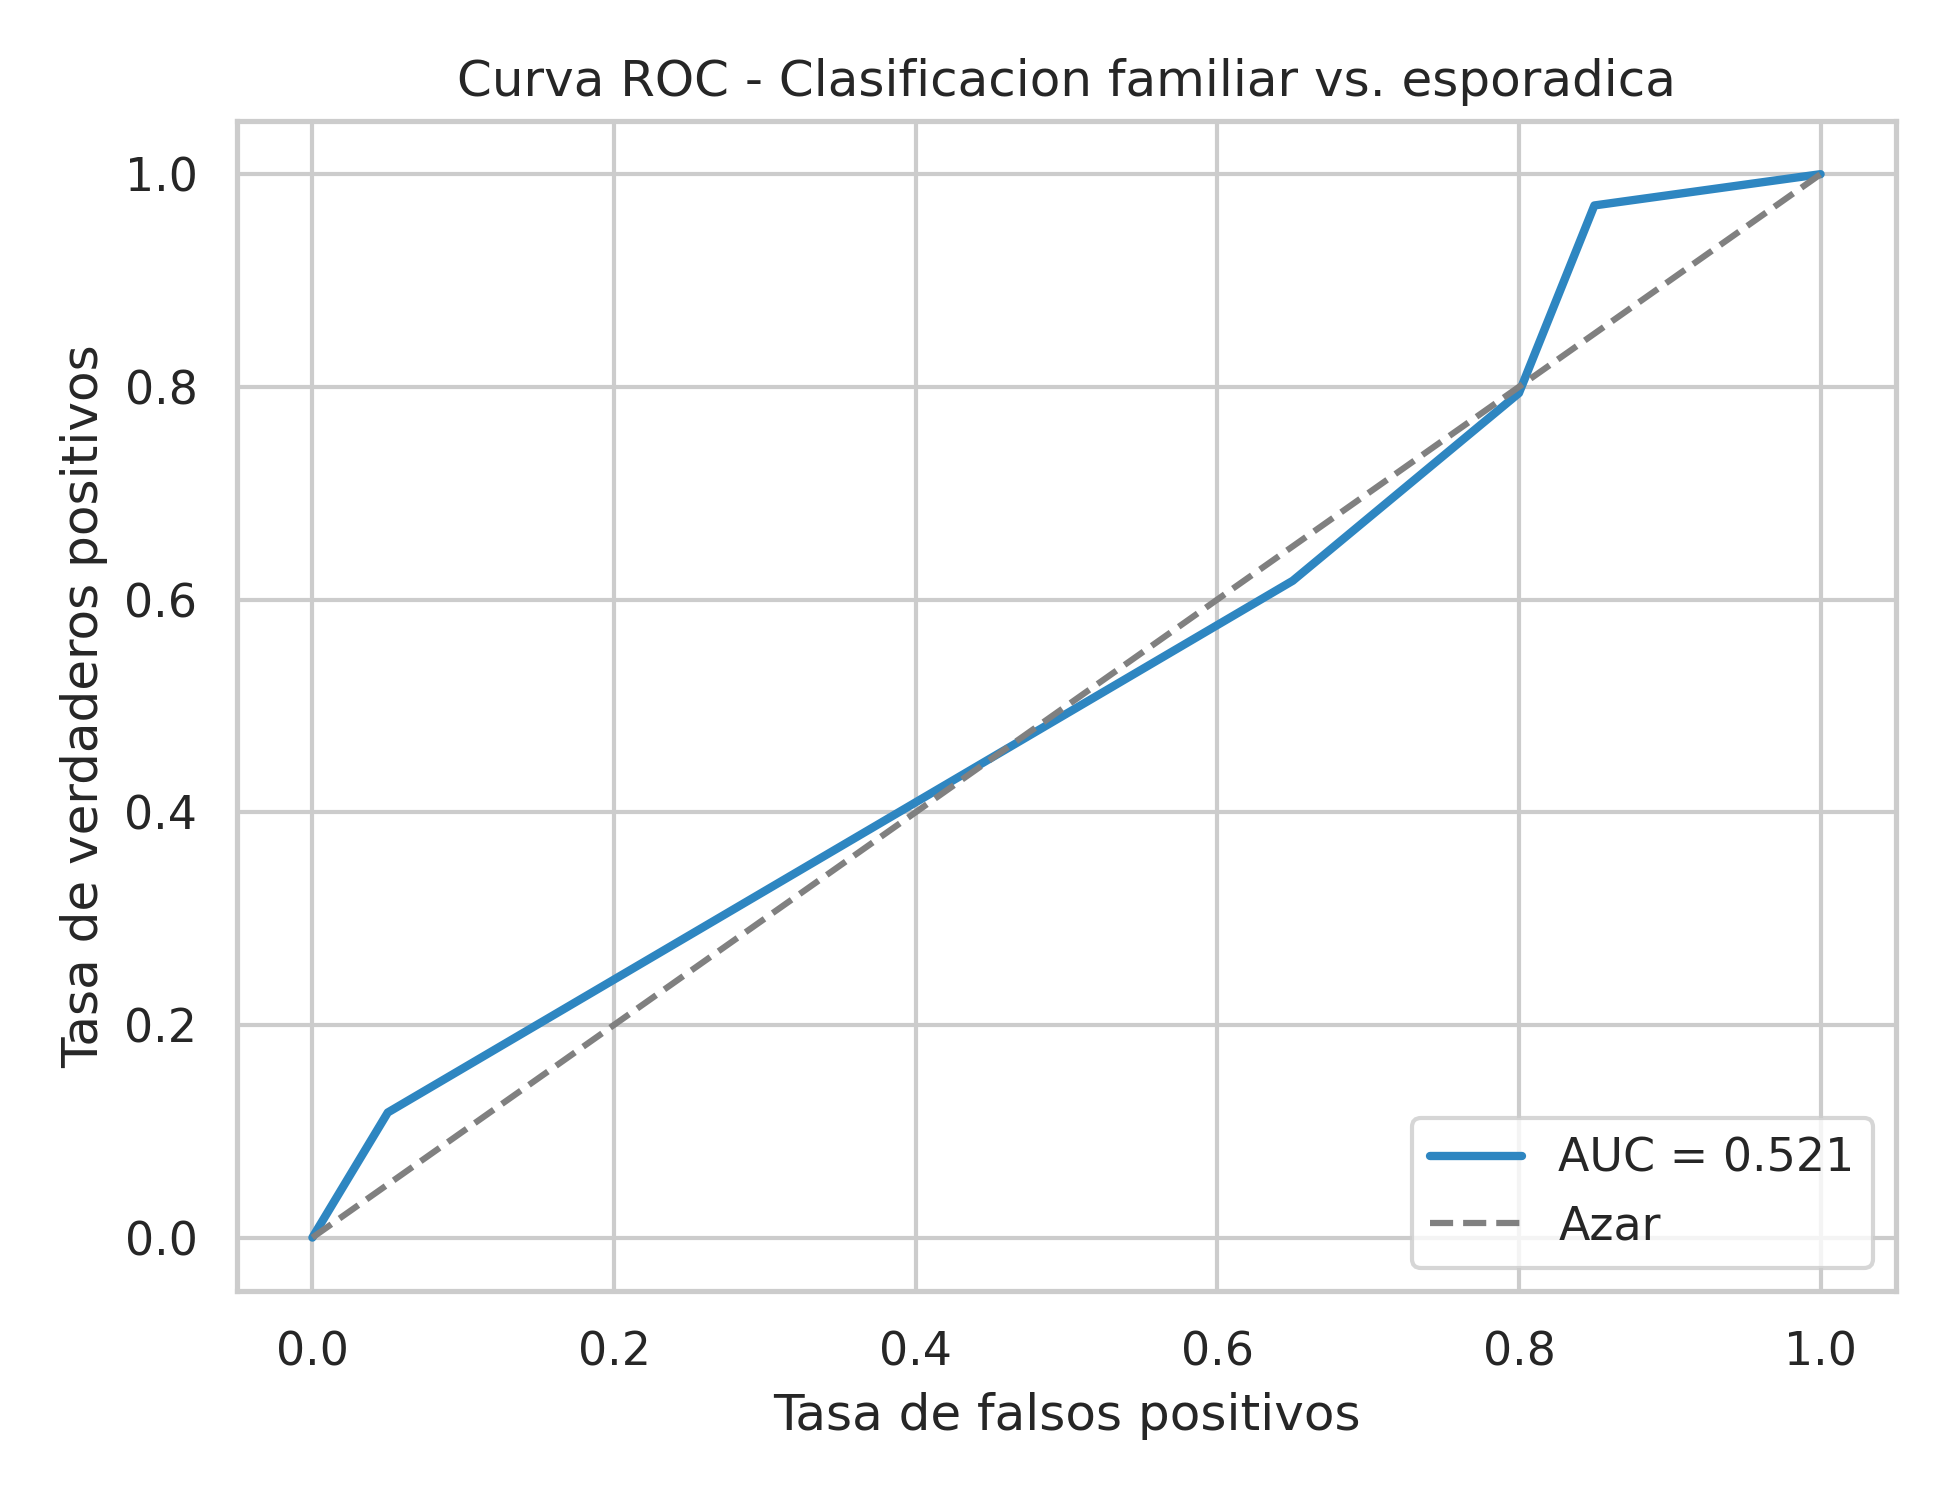
\includegraphics[width=0.62\textwidth]{figuras/curva_roc.png}
\caption{Curva ROC del arbol de decision.}
\label{fig:curva_roc}
\end{figure}

\begin{table}[H]
\centering
\small
\begin{tabular}{lrr}
\toprule
Metrica en validacion cruzada & Media & Desv. estandar \\
\midrule
Accuracy & 0,524 & 0,036 \\
Precision & 0,487 & 0,022 \\
Recall & 0,667 & 0,174 \\
F1-score & 0,549 & 0,078 \\
AUC-ROC & 0,528 & 0,041 \\
\bottomrule
\end{tabular}
\caption{Validacion cruzada estratificada de cinco pliegues.}
\label{tab:cv}
\end{table}

La validacion cruzada entrega un F1 promedio de 0,549 y recall promedio de 0,667 para la clase familiar, pero el AUC promedio sigue bajo. Esto sugiere que hay senales debiles o no lineales, y que un solo arbol puede ser insuficiente para capturar la relacion entre sintomas y tipo de caso.

\section{Conclusiones y Discusion}

El analisis permitio aplicar CRISP-DM de forma completa: se definio el objetivo de clasificacion, se reviso la estructura del Excel, se imputaron valores faltantes, se entreno un arbol de decision y se evaluo con metricas de prueba y validacion cruzada. El dataset local contiene 296 registros, menos que los 331 indicados en la descripcion general de UCI, por lo que las conclusiones se restringen al archivo efectivamente analizado.

Los hallazgos principales son prudentes. Las diferencias descriptivas entre casos familiares y esporadicos existen, pero son pequenas. La presencia de tumores fue algo mayor en familiares (30,4\%) que en esporadicos (25,5\%), mientras que nodulos de Lisch fueron mas frecuentes en esporadicos. En el modelo, las variables usadas por el arbol fueron principalmente edad al primer diagnostico, nodulos de Lisch, glioma optico y edad de la madre. La variable \texttt{Tumour Case} no quedo entre las divisiones del arbol final, aunque descriptivamente si muestra una diferencia leve entre grupos.

El desempeno predictivo es limitado. El AUC cercano a 0,52 indica que el arbol apenas separa las clases mejor que una decision aleatoria. Esto no invalida la tarea, pero obliga a interpretar el modelo como herramienta pedagogica e interpretativa. En salud, un resultado de este nivel no debe usarse para decisiones clinicas. Posibles mejoras incluyen validar con mas datos, revisar codificacion clinica, probar Random Forest, XGBoost o Gradient Boosting, ajustar umbrales de decision y considerar interacciones no capturadas por un arbol pequeno.

Juan Muñoz concluye que CRISP-DM ayudo a ordenar el problema desde la pregunta clinica hasta la evaluacion, evitando saltar directamente al modelo. La principal evidencia fue que la preparacion de datos y la revision de clases condicionan toda lectura posterior.

Vicente Rivera concluye que las visualizaciones de distribucion y prevalencia son claves para interpretar el dataset antes de modelar. En particular, las diferencias entre sintomas existen, pero no son suficientemente fuertes para sostener afirmaciones clinicas deterministas.

Fernando Valdés concluye que el arbol de decision es valioso por su interpretabilidad, aunque sus metricas muestran limites claros. Para mejorar la capacidad predictiva se requeririan modelos de ensamble y validacion externa.

Como conclusion general, el trabajo cumple el objetivo de investigar y aplicar arboles de decision en un problema de clasificacion con datos reales de NF1. Su aporte principal es una implementacion reproducible, una evaluacion honesta y una discusion metodologica alineada con la naturaleza exploratoria del dataset.

\section*{Declaracion de elaboracion y apoyo}

El informe, el analisis de datos y la interpretacion de resultados fueron elaborados por el grupo. Se utilizo GPT 5.5 como herramienta de apoyo editorial y de asistencia en programacion para revisar consistencia formal, redaccion y estructura reproducible. El contenido, los resultados y las conclusiones fueron revisados y validados por los autores del informe.

\begin{thebibliography}{99}

\bibitem{chapman2000}
Chapman, P., Clinton, J., Kerber, R., Khabaza, T., Reinartz, T., Shearer, C. y Wirth, R. (2000). \textit{CRISP-DM 1.0: Step-by-Step Data Mining Guide}. SPSS Inc.

\bibitem{breiman1984}
Breiman, L., Friedman, J., Olshen, R. y Stone, C. (1984). \textit{Classification and Regression Trees}. Wadsworth.

\bibitem{uci2025nf1}
UCI Machine Learning Repository. (2025). \textit{Neurofibromatosis Type 1: Clinical Symptoms of Familial and Sporadic Cases}. Disponible en: \url{https://archive.ics.uci.edu/dataset/1162/neurofibromatosis+type+1+clinical+symptoms+of+familial+and+sporadic+cases}

\bibitem{sharafi2025nf1}
Sharafi, P., Arslan, H., Ersoy Evans, S., Varan, A. y Ayter, S. (2025). A machine learning approach for predicting familial and sporadic disease cases based on clinical symptoms: introduction of a new dataset. \textit{Turkish Bulletin of Hygiene and Experimental Biology}.

\bibitem{sklearn2011}
Pedregosa, F. et al. (2011). Scikit-learn: Machine Learning in Python. \textit{Journal of Machine Learning Research}, 12, 2825--2830.

\bibitem{pandas2020}
The pandas development team. (2020). \textit{pandas-dev/pandas: Pandas}. Zenodo. \url{https://doi.org/10.5281/zenodo.3509134}

\bibitem{hunter2007}
Hunter, J. D. (2007). Matplotlib: A 2D Graphics Environment. \textit{Computing in Science \& Engineering}, 9(3), 90--95.

\bibitem{waskom2021}
Waskom, M. (2021). Seaborn: Statistical Data Visualization. \textit{Journal of Open Source Software}, 6(60), 3021.

\bibitem{levano2026}
Lévano, M. (2026). Material de clase INFO1184 Inteligencia de Negocios: CRISP-DM, modelamiento y evaluacion. Universidad Catolica de Temuco.

\end{thebibliography}

\appendix
\section{Anexo: Reproducibilidad y Bitacora}

El analisis se reproduce ejecutando \texttt{nf1\_analisis.py} desde la carpeta \texttt{TA06/}. El script genera automaticamente las seis figuras usadas en el informe dentro de \texttt{figuras/}. La Tabla~\ref{tab:archivos} resume los archivos principales.

\begin{table}[H]
\centering
\small
\begin{tabularx}{\textwidth}{p{5.2cm}X}
\toprule
Archivo & Descripcion \\
\midrule
\texttt{dataset-uci.xlsx} & Excel local con hoja \texttt{Dataset}. \\
\texttt{nf1\_analisis.py} & Script reproducible de carga, preparacion, modelado, evaluacion y figuras. \\
\texttt{figuras/arbol\_decision.png} & Visualizacion del arbol entrenado. \\
\texttt{figuras/matriz\_confusion.png} & Matriz de confusion del conjunto de prueba. \\
\texttt{figuras/curva\_roc.png} & Curva ROC y AUC del modelo. \\
\texttt{figuras/importancia\_features.png} & Ranking de importancia de variables. \\
\texttt{figuras/distribucion\_clases.png} & Balance de clases objetivo. \\
\texttt{figuras/prevalencia\_sintomas.png} & Prevalencia de sintomas por tipo de caso. \\
\bottomrule
\end{tabularx}
\caption{Estructura de archivos principales de TA06.}
\label{tab:archivos}
\end{table}

\begin{table}[H]
\centering
\small
\begin{tabularx}{\textwidth}{p{2.8cm}p{3.6cm}X}
\toprule
Etapa & Responsable principal & Actividad \\
\midrule
Comprension & Juan Muñoz & Revision de enunciado, objetivo y enfoque CRISP-DM. \\
Datos & Vicente Rivera & Revision de columnas, faltantes, clases y prevalencias. \\
Modelado & Fernando Valdés & Implementacion del arbol de decision, validacion y metricas. \\
Visualizacion & Grupo completo & Generacion y revision de figuras explicativas. \\
Informe & Grupo completo & Redaccion, discusion, conclusiones y revision final. \\
\bottomrule
\end{tabularx}
\caption{Bitacora resumida del trabajo.}
\label{tab:bitacora}
\end{table}

\end{document}
